\documentclass[a4paper, DIV11, abstracton]{scrartcl}
\usepackage{color,graphicx}			% graphics package

\usepackage{microtype}				% optical margin alignment
\usepackage[T1]{fontenc}			% umlauts for european languages
\usepackage{textcomp}				% provides extra symbols
\usepackage[utf8]{inputenc}			% character encoding
\usepackage[USenglish]{babel}		% elements language and hyphenation

\usepackage[round]{natbib}			% scientific bibliography
%\usepackage{url}					% nicely spaced urls
\usepackage{amsmath}				% mathematical equation alignment
%\usepackage{dcolumn}				% decimal alignment in tables
\usepackage{siunitx}				% units (micrometers, anyone?)
\usepackage[font=small, format=plain, labelsep=period, labelfont={sf,bf}, justification=justified]{caption}	% formatting the labels for figures, tables

% fonts
\usepackage{palatino}
\usepackage{mathpazo}
\usepackage[scaled=0.92]{helvet}

% matlab code
\usepackage[numbered,autolinebreaks,framed]{mcode}

% spacing
\setlength{\parskip}{0.2cm}			% remove indent at paragraphs
\setlength{\parindent}{0pt}			% remove indent at paragraphs
\renewcommand{\baselinestretch}{1.1}	% control line spacing in text

\setcounter{secnumdepth}{2}			% only number top headings (\section)
\setcounter{tocdepth}{2}			% include \subsection in TOC

\usepackage[raiselinks, pdfborder={0 0 0}]{hyperref}  % creates pdf sections for acrobat
%\hypersetup{pdftitle={Title}}



\begin{document}
\thispagestyle{empty}




%\thispagestyle{empty} % no page numbers on title page
Lecture with Computer Exercises: Modelling and Simulating Social Systems with MATLAB
Project Report

Document Version: 1.0\\*
Group Name: Rieparjo\\*
Group Members: Christoph Rieper and Benjamin Sunarjo



\newpage
\setcounter{page}{1}
\pagenumbering{roman}
%=-=-=-=-=-=-=-=-=-=-=-=-=-=-=-=-=-=-=-=-=-=-=-=-=-=-=-=-=-=-=-=-=-=
\section*{Agreement for free-download}
%=-=-=-=-=-=-=-=-=-=-=-=-=-=-=-=-=-=-=-=-=-=-=-=-=-=-=-=-=-=-=-=-=-=

We hereby agree to make our source code for this project freely available for download from the web pages of the SOMS chair. Furthermore, we assure that all source code is written by ourselves and is not violating any copyright restrictions.

\bigskip
Christoph Rieper

\bigskip
Benjamin Sunarjo

\newpage


\tableofcontents

\newpage
\setcounter{page}{1}	% start page numbering here
\pagenumbering{arabic}
\pagestyle{plain}
%=-=-=-=-=-=-=-=-=-=-=-=-=-=-=-=-=-=-=-=-=-=-=-=-=-=-=-=-=-=-=-=-=-=
\section*{Abstract}
%=-=-=-=-=-=-=-=-=-=-=-=-=-=-=-=-=-=-=-=-=-=-=-=-=-=-=-=-=-=-=-=-=-=

%=-=-=-=-=-=-=-=-=-=-=-=-=-=-=-=-=-=-=-=-=-=-=-=-=-=-=-=-=-=-=-=-=-=
\section*{Individual contributions}
%=-=-=-=-=-=-=-=-=-=-=-=-=-=-=-=-=-=-=-=-=-=-=-=-=-=-=-=-=-=-=-=-=-=


%=-=-=-=-=-=-=-=-=-=-=-=-=-=-=-=-=-=-=-=-=-=-=-=-=-=-=-=-=-=-=-=-=-=
\section{Introduction}
%=-=-=-=-=-=-=-=-=-=-=-=-=-=-=-=-=-=-=-=-=-=-=-=-=-=-=-=-=-=-=-=-=-=

%(States your motivation clearly: why is it important / interesting to solve this problem?)
%(Add real-world examples, if any)
%(Put the problem into a historical context, from what does it originate? Are there already some proposed solutions?)

Agent-based models can provide a easily implementable way to study complex systems. As \citet{helbing:1997} have shown, many aspects of pedestrian motion, such as the formation of trail systems in green areas, can be reproduced using a relatively simple ``active walker'' model that takes into account the attractiveness of terrain and feedback on the terrain as it is walked upon. In the current project, we plan to apply such an active walker model to real landscapes and compare the results to existing road systems.



%(At the end of the project you want to find the answer to these questions)
%(Formulate a few, clear questions. Articulate them in sub-questions, from the more general to the more specific. )
%(Define dependent and independent variables you want to study. Say how you want to measure them.)

We attempt to answer the question: is the active walker model able to predict reasonable pathways between neighboring villages in real landscapes? Here, ``reasonable'' will be evaluated first in a qualitative sense. Second, a energy function will be defined based on the distance traveled horizontally and vertically, where a minimal energy function is most reasonable.

In a second step, we will determine the influence of landscape slope on trail formation, under the assumption that modern roads are situated where historically trails used to go through. We will compare generated paths to current road networks at two test sites to answer the questions: How does trail formation change with increasing landscape slope? Do the formed paths fit to current road networks?

Theoretical work by \citet{helbing:1997} has previously been implemented in an agent-based model by \citet{trailsystems}. We will base our investigation of the above research questions on this model, making adjustments where necessary. We will use topographical data from swisstopo.admin.ch with an emphasis on 1. determining reasonable model parameters and 2. comparing modeled trails to existing road systems. Two test sites are proposed, one in an mountainous region in St. Moritz, the other in the Swiss lowlands near Friburg (Figure~\ref{fig:site}). These two test sites provide very different types of terrain on which to study the problem of trail formation.

\begin{figure}[tbp]
	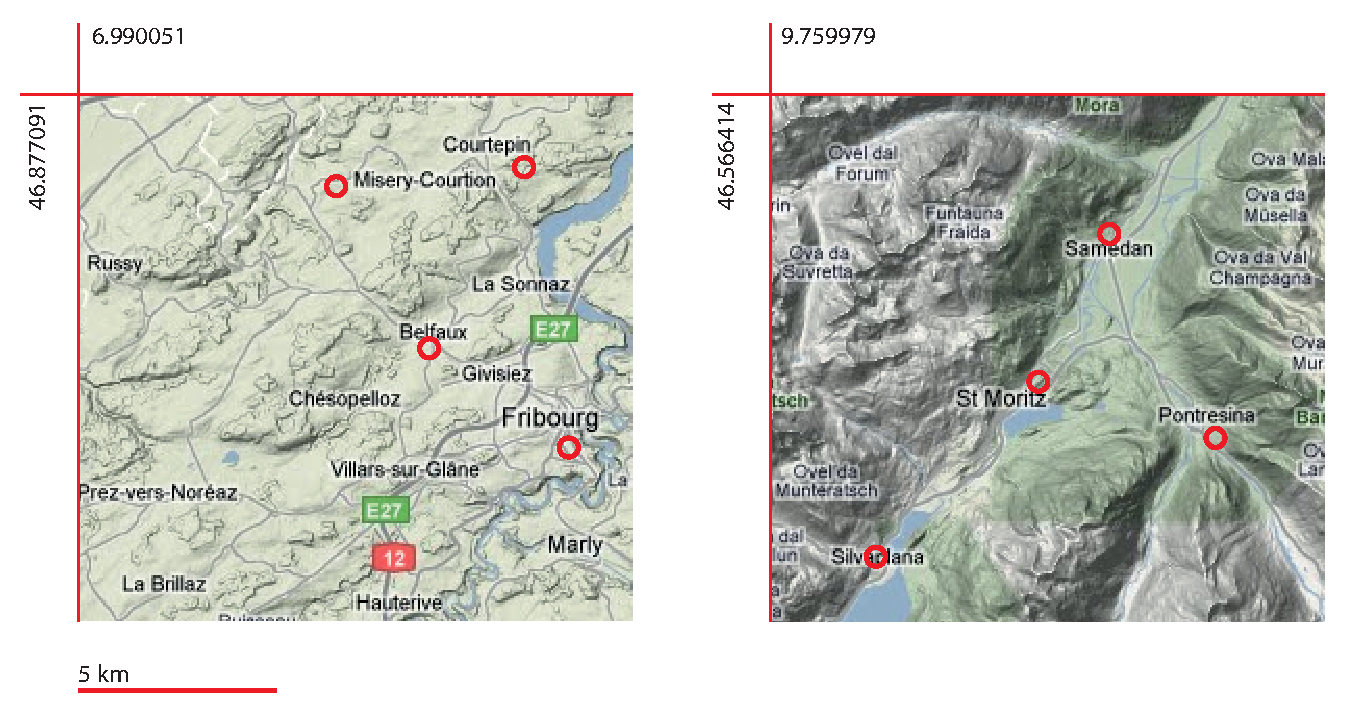
\includegraphics[width=\linewidth]{../figures/site}
	\caption{Two test sites, one mountainous one flat.}
	\label{fig:site}
\end{figure}

We expect to find that the smaller roads correspond more closely to results generated by the active walker model, while larger cantonal roads, being further removed from their trail origins, should correspond less with model results. We further expect increasingly mountainous terrain to tightly constrain possible routes: we expect closer correlation between road systems and generated model results in mountainous regions than in the lowlands, since there are less possibilities for taking a route with low associated energy cost.


\subsection{site}




\section{Description of the Model}

Our studies are based on an active walker model developed by \cite{helbing:1997}. \cite{helbing:1997} used this agent-based model to explain footpath formation in green areas in cities.

In comparison to a normal pedestrian model, an active walker model also takes the interactions of the pedestrians and the terrain they walked upon into account. This means that the pedestrians change the landscape they walk upon and the changed landscape influences again the pedestrians movement. A second important characteristic of the model, which influences the direction of walking of the pedestrians, is the attractiveness of a trail segment. It is a property of each point in the terrain, which describes how interesting it is to go to this certain place. In other words, how good the prospects are on this place for further walking. It is the element of our model which handles the effect of human orientation and is described later on in more detail.

As the model consists of three major components (the ground, the attractiveness of a trail segment and the pedestrians), all three are described separately. The ground and the influence of the pedestrians on it is described in Sec.\ \ref{ground_structure}. Sec.\ \ref{trail_potential} explains how the attractiveness of walking is computed and Sec.\ \ref{pedestrians_direction} illustrates how the pedestrians walking direction is determined.

\subsection{Ground Structure}
\label{ground_structure}

Our landscape is represented by a function $G(r,t)$, called comfort of walking, with $r$ for the position in the plane and $t$ for time. As it is a property of our plane it is defined on each point. High values of $G$ stand for trails, i.e. places where many people walked upon, while low values of $G$ stand for places where fewer people passed by. Every time a pedestrian walks on o certain point of the plain it changes the comfort of walking there. This is because pedestrians trample down the vegetation. This is described by

\begin{equation}
\label{trample_down}
I(r)[1-\frac{G(r,t)}{G_{max}(r)}]\ ,
\end{equation}

where $I(r)$ stands for the intensity of the footprint and $G_{max}(r)$ for the maximal value of the comfort of walking at a certain place (i.e. the maximal value a place can be trampled "up"). The expression in the brackets of Eq.\ \ref{trample_down} account for the saturation effect, so that the impact of the footprints decreases when there are more people walking on a place until the maximal value is reached.

As the vegetation can be trampled down it can also regrow. This effect is expressed by

\begin{equation}
\frac{1}{T(r)}[G_0(r)-G(r,t)]
\end{equation}

where $G_0(r)$ stands for the natural ground condition and $T(r)$ for the durability of the trails. The bigger the durability $T(r)$ the slower the ground goes back to natural conditions $G_0(r)$.

Finally the change of the comfort of walking by time due to the walking pedestrians and the regrowth of the vegetation can be expressed as

\begin{equation}
\frac{dG(r,t)}{dt}=I(r)[1-\frac{G(r,t)}{G_{max}(r)}]\sum\limits_{\alpha} \delta(r-r_{\alpha}(t)) +\frac{1}{T(r)}[G_0(r)-G(r,t)]
\end{equation}

with $\alpha$ for the set of pedestrians and $\delta(r-r_{\alpha}(t))$ standing for the Dirac delta function, which is 1 if $r=r_(\alpha)$ and 0 in all other cases and therefore only contributs if a pedestrian is on the actual position.

\subsection{Attractiveness of Trail Segment}
\label{trail_potential}

As mentioned above the attractiveness of a trail segment is a measure of how interesting a place is in manner of later onward walking. It is defined for every place and depends on the comfort of walking of its surrounding, where the influence of the surround decreases with distance from the place. The attractiveness of a trail segment is called trail potential and is defined as

\begin{equation}
V_{tr}(r_t,t) = \int_{P} G(r,t) e^{\frac{-|r-r_t|}{\sigma(r_t)}} dP
\end{equation}

where $r_t$ stands for the position the trail potential is computed for, P for the plain and $\sigma(r_t)$ for the visibility. The visibility controls how fast the influence of the surrounding decreases. The higher the visibility the slower the influence of the surrounding decreases. Furthermore high values of the trail potential stand for a high attractiveness of a trail segment and vice versa. 

\subsection{Pedestrians Walking Direction}
\label{pedestrians_direction}

In the model every pedestrian has a starting point and a destination. When the pedestrians walking direction is determined two vectors decide about the final walking direction. One vector is the vector which points towards the pedestrians destination. It is given by the unit vector

\begin{equation}
\label{dest_1}
e_{\alpha}^{1}(r_{\alpha},t)=\frac{d_{\alpha}-r_{\alpha}}{|d_{\alpha}-r_{\alpha}|}
\end{equation}

where $d_{\alpha}$ is the position of the pedestrians destination.The other vector which decides about the pedestrians walking direction is the vector which points into the direction of highest increase of the trail potential. It can be expressed in the normalized form as

\begin{equation}
\label{dest_2}
e_{\alpha}^{2}(r_{\alpha},t)=\frac{\nabla{V_{tr}(r_{\alpha},t)}}{|\nabla{V_{tr}(r_{\alpha},t)}|}.
\end{equation}

Combining Eq.\ \ref{dest_1} and \ref{dest_2} and introducing a new variable $\rho$ that controls the relative importance of the two vectors leads to the final walking direction

\begin{equation}
e_{\alpha}(r_{\alpha},t)=\rho \cdot e_{\alpha}^{1}(r_{\alpha},t)+e_{\alpha}^{2}(r_{\alpha},t)=\rho \cdot \frac{d_{\alpha}-r_{\alpha}}{|d_{\alpha}-r_{\alpha}|}+\frac{\nabla{V_{tr}(r_{\alpha},t)}}{|\nabla{V_{tr}(r_{\alpha},t)}|}.
\end{equation}

For value of $\rho>1$ the destination vector gets more important and for value $\rho<1$ the direction of the highest increase of the trail potential prevails.

\section{Description of the Path-Evaluation Function}

To evaluate the paths taken by the pedestrians a function was defined to judge if a path is reasonable or not. As described by \citet{koelbl_helbing:2003} humans try to minimize their cost of travel. Cost of travel in our case is travel-time. Therefore we developed a function which calculates the time it needs to walk a certain path.

Assuming a horizontal speed $u_{horiz}(G(r_{\alpha},t))$ which scales with comfort of walking and a constant vertical speed $u_{vert}$ the travel-time is given by

\begin{equation}
T= \frac{s_{horiz}}{u_{horiz}(G(r_{\alpha},t))} + \frac{s_{vert}}{u_{vert}} \,,
\end{equation}

where $s_{vert}$ is the uphill travelled distance and $s_{horiz}$ the horizontally traveled distance. In more detail the horizontal speed $u_{horiz}$ scales between a minimal horizontal speed $u_{horiz,min}$ and a maximal horizontal speed $u_{horiz,max}$ depending on how strongly the path is trampled down. This is expressed as

\begin{equation}
u_{horiz}(r_{\alpha},t) = u_{horiz,min} + (u_{horiz,max}-u_{horiz,min}) \cdot \frac{G(r_{\alpha},t)-G_{0}(r_{\alpha},t)}{G_{max}(r_{\alpha},t)-G_{0}(r_{\alpha},t)}.
\end{equation}

In Tab.\ \ref{table_speed} values of $u_{horiz,min}$, $u_{horiz,max}$ and $u_{vert}$ which are used in the path-evaluation function can be found.

\begin{table}[h]
\begin{center}
 \setlength{\abovecaptionskip}{0pt}
 \setlength{\belowcaptionskip}{10pt}
\caption{Vertical and horizontal speed used in path-evaluation function.}
\begin{tabular}{c l l}
  \hline
  $u_{horiz,min}$ & $u_{horiz,max}$ & $u_{vert}$ \\
  4000 $m\,h^{-1}$ & 6000 $m\,h^{-1}$ & 500 $m\,h^{-1}$ \\ \hline
\end{tabular}
\label{table_speed}
\end{center}
\end{table}
\section{Implementation}

The active walker model was previously implemented by \citet{trailsystems}. We further developed the model by adding the path-evaluation function and the interface to work with real elevation data to its functionalities. The implementation by \citet{trailsystems} is described in their report, while our contribution is described here.

\subsection{Interface for real Elevation Data}

The elevation data provided by swisstopo.admin.ch (5$\times$5 $km$ for each site) came in a resolution of 25$\times$25 $m$. To use this elevation data in our model first the resolution had to to be lowered to 500$\times$500 $m$ for computational reasons and then the data had to be adjusted to use it as initial comfort of walking $G_0$.

As high values of comfort of walking represent paths which are favored for walking on and high values in the elevation data are mountains which are not favored for walking on the elevation model had to be inverted. So in the inverted elevation model valleys became  mountains and mountains became valleys. Therefore the initial comfort of walking was set to

\begin{equation}
G_0 = argMax(E)-E \,
\end{equation}

where E is the original elevation model.

\subsection{Implementation of the Path-Evaluation Function}

To add the path-evaluation function to the model the pedestrian class had to be changed and a new class, the path class was created. First the changes to the pedestrian class are described followed by the introduction of the path class.

To evaluate the travel-time equation (Eq.\ \ref{eq:time}) the relative ground $\frac{G(r_{\alpha},t)-G_{0}(r_{\alpha},t)}{G_{max}(r_{\alpha},t)-G_{0}(r_{\alpha},t)}$ and the coordinates of the walked way by the pedestrian have to be known. Therefore the pedestrian class was changed to save the coordinates and the relative ground on this coordinates on every time step of the state machine.

Furthermore on every time step when a pedestrian arrives at his destination the information about the walked path is used the create an object of the new path class. An object of the path class has the following properties: coordinates, relative ground on coordinates, time, time of arrival and type. The coordinates and the relative ground on the coordinates are provided by the pedestrian object itself while time is the result of the travel-time equation and time of arrival the time step in which the state machine is in when the pedestrian arrives. The type of the path is a number which was assigned to the path depending on which way (which start and which destination) the pedestrian went. All the created path objects are then saved in the simulation for later analysis.

%=-=-=-=-=-=-=-=-=-=-=-=-=-=-=-=-=-=-=-=-=-=-=-=-=-=-=-=-=-=-=-=-=-=
\section{Simulation Results and Discussion}
%=-=-=-=-=-=-=-=-=-=-=-=-=-=-=-=-=-=-=-=-=-=-=-=-=-=-=-=-=-=-=-=-=-=
In our analysis of the path formation process using our active walker model, the biggest uncertainty concerned the values of the various independent parameters (durability and intensity of trails, visibility, relative importance of the destination vector). No literature values could be found for these values (they are dependent on model specifics such as the model scale). Since our initial hypotheses cannot be conclusively addressed without first dealing with the issue of model parameters, we first discuss the effects parameter variation has on model results, then look in detail at the generated path structures. Finally, we compare our results with existing road structures.

%=-=-=-=-=-=-=-=-=-=-=-=-=-=-=-=-=-=-=-=-=-=-=-=-=-=-=-=-=-=-=-=-=-=
\subsection{Parameter variation}

\subsubsection{visibility}

\subsubsection{importance}

\subsubsection{durability}

\subsubsection{intensity}


%=-=-=-=-=-=-=-=-=-=-=-=-=-=-=-=-=-=-=-=-=-=-=-=-=-=-=-=-=-=-=-=-=-=
\subsection{Path structure}


%=-=-=-=-=-=-=-=-=-=-=-=-=-=-=-=-=-=-=-=-=-=-=-=-=-=-=-=-=-=-=-=-=-=
\subsection{Existing road structure}

\begin{figure}[tbp]
	\includegraphics[width=\linewidth]{../figures/roads}
	\caption{The road structure at the two study sites (A: Fribourg, B: St. Moritz). Coordinates are given in the reference frame CH1903. The line weight is derived from road class order (highways and 1. order roads are heavier in weight than higher order roads; see \citet{vector25}) and does not necessarily correlate to throughput.}
	\label{fig:roads}
\end{figure}

qualitative differences between the two sites. Road structure at the St. Moritz site shows close similarity to the structure of alpine rivers, 




%=-=-=-=-=-=-=-=-=-=-=-=-=-=-=-=-=-=-=-=-=-=-=-=-=-=-=-=-=-=-=-=-=-=
\section{Summary and Outlook}
%=-=-=-=-=-=-=-=-=-=-=-=-=-=-=-=-=-=-=-=-=-=-=-=-=-=-=-=-=-=-=-=-=-=
We found:
-it's most important to determine correct parameter values
-there are qualitative differences between the two study sites.

%=-=-=-=-=-=-=-=-=-=-=-=-=-=-=-=-=-=-=-=-=-=-=-=-=-=-=-=-=-=-=-=-=-=
%\addcontentsline{toc}{section}{References}  % adds references section to TOC
%\bibliographystyle{apalike2}
%\bibliography{references}

\renewcommand{\refname}{\section{References}} % Using "Sources" as the title of the section
\bibliographystyle{apalike2}
\bibliography{references}


\newpage
%=-=-=-=-=-=-=-=-=-=-=-=-=-=-=-=-=-=-=-=-=-=-=-=-=-=-=-=-=-=-=-=-=-=
\section{Appendix: Matlab Code}
%=-=-=-=-=-=-=-=-=-=-=-=-=-=-=-=-=-=-=-=-=-=-=-=-=-=-=-=-=-=-=-=-=-=
\subsection*{batch.m}
\lstinputlisting{../matlab/batch.m}
\subsection*{Path.m}
\lstinputlisting{../matlab/Path.m}
\subsection*{Pedestrian.m}
\lstinputlisting{../matlab/Pedestrian.m}
\subsection*{Plain.m}
\lstinputlisting{../matlab/Plain.m}
\subsection*{smDriver.m}
\lstinputlisting{../matlab/smDriver.m}
\subsection*{StateMachine.m}
\lstinputlisting{../matlab/StateMachine.m}
\subsection*{visualization.m}
\lstinputlisting{../matlab/visualization.m}


\end{document}
